\section{相关高斯噪声}
\label{sec:gcc-correlated}

平行信道假设各分量的噪声互相独立。两条并排的线路常常受到同一个干扰源的影响，噪声会相关。设两条线路的噪声方差都是$2$，协方差是$1$，即
\[
 \bm{Z}\sim\mathcal{N}(\bm{0},\bm{\Sigma}),\qquad \bm{\Sigma}=\begin{bmatrix}2&1\\1&2\end{bmatrix},
\]
总功率预算为$P=2$。这时各分量不能单独处理，注水规则还能用吗？功率应当分给哪个方向？

\paragraph{模型}
设$\bm{\Sigma}$是$k\times k$实对称正定矩阵。每次使用时输入$\bm{x}_i\in\mathbb{R}^k$，输出
\begin{equation}
 \bm{Y}_i=\bm{x}_i+\bm{Z}_i,\qquad \bm{Z}_1,\dots,\bm{Z}_n\ \text{独立同分布},\ \bm{Z}_i\sim\mathcal{N}(\bm{0},\bm{\Sigma}),
 \label{eq:gcc-correlated}
\end{equation}
噪声与消息独立。码字满足欧氏总能量约束$\sum_{i=1}^{n}\lVert\bm{x}_i(m)\rVert_2^2\leq nP$。同一时刻各分量的噪声可以相关，不同时刻之间仍然独立。

\paragraph{正交变换}
由谱分解（\BookChapterRef{chap:eigen-spectral-decomposition}{卷二第6章“谱分解”}），$\bm{\Sigma}=\bm{U}\bm{\Lambda}\bm{U}^{\top}$，其中$\bm{U}$是正交矩阵，列向量$\bm{u}_1,\dots,\bm{u}_k$是$\bm{\Sigma}$的单位特征向量，$\bm{\Lambda}$是以特征值$\lambda_1,\dots,\lambda_k$为对角元的对角阵，正定性保证每个$\lambda_j>0$。在特征向量的坐标下看噪声：
\[
 \tilde{\bm{Z}}=\bm{U}^{\top}\bm{Z}\sim\mathcal{N}\bigl(\bm{0},\bm{U}^{\top}\bm{\Sigma}\bm{U}\bigr)=\mathcal{N}(\bm{0},\bm{\Lambda}) .
\]
$\tilde{\bm{Z}}$的协方差矩阵是对角阵，各分量不相关；它们又是联合高斯的，由第~\ref{chap:multivariate-distributions}章，不相关的联合高斯分量相互独立。所以在这组坐标下，噪声变成了方差为$\lambda_1,\dots,\lambda_k$的独立分量。

同一组坐标也保持功率预算：$\bm{U}$是正交矩阵，对任意$\bm{x}\in\mathbb{R}^k$，
\[
 \lVert\bm{U}^{\top}\bm{x}\rVert_2=\lVert\bm{x}\rVert_2 .
\]
噪声变得独立、预算形式不变，这两点合起来说明相关噪声信道与平行信道等价。

\begin{lemma}[正交坐标下的等价]
\label{lem:gcc-rotation}
对式~\eqref{eq:gcc-correlated}的信道，记噪声方差为$\lambda_1,\dots,\lambda_k$的平行信道为$\tilde{\mathcal{C}}$。满足功率约束$P$的$(M,n)$码在两个信道之间可以一一对应，对应的码满足同样的约束，并且每条消息的条件错误概率相同。
\end{lemma}

\begin{proof}
设$(\tilde{f},\tilde{g})$是$\tilde{\mathcal{C}}$上的码，消息$m$的码字由$n$个向量$\tilde{\bm{x}}_i(m)$组成，$i=1,\dots,n$。在相关噪声信道上，令编码器发送$\bm{x}_i(m)=\bm{U}\tilde{\bm{x}}_i(m)$，解码器先把每个输出向量乘以$\bm{U}^{\top}$，再用$\tilde{g}$判决。能量逐时刻保持，所以约束成立。发送消息$m$时，
\[
 \bm{U}^{\top}\bm{Y}_i=\tilde{\bm{x}}_i(m)+\bm{U}^{\top}\bm{Z}_i ,
\]
$\bm{U}^{\top}\bm{Z}_1,\dots,\bm{U}^{\top}\bm{Z}_n$独立同分布于$\mathcal{N}(\bm{0},\bm{\Lambda})$，所以$\tilde{g}$看到的输入与在$\tilde{\mathcal{C}}$上看到的分布完全相同，条件错误概率相同。反方向把$\bm{U}$与$\bm{U}^{\top}$对调即可。
\end{proof}

图~\ref{fig:gcc-rotation-equivalence}画出这个对应：发送端和接收端各乘一个正交矩阵，中间的相关噪声信道在外面看来就是平行信道。

\begin{BookInlineFigure}
 \centering
 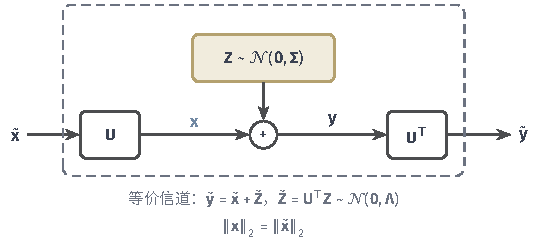
\includegraphics[width=90mm]{figures/07-probability/06-channel-coding/tikz/gcc-rotation-equivalence/figure.pdf}
 \caption{相关噪声信道与平行信道的等价。发送端把$\tilde{\bm{x}}$变成$\bm{x}=\bm{U}\tilde{\bm{x}}$，信道加上噪声$\bm{Z}\sim\mathcal{N}(\bm{0},\bm{\Sigma})$（黄框），接收端乘以$\bm{U}^{\top}$。虚线框整体是噪声方差为$\lambda_1,\dots,\lambda_k$的平行信道，正交变换保持欧氏长度。}
 \label{fig:gcc-rotation-equivalence}
\end{BookInlineFigure}

由引理~\ref{lem:gcc-rotation}和定理~\ref{thm:gcc-parallel-coding}，相关噪声信道的容量就是对特征值$\lambda_1,\dots,\lambda_k$注水得到的值。最优输入也可以写回原坐标。

\begin{theorem}[相关高斯噪声信道的容量]
\label{thm:gcc-correlated}
设$\bm{\Sigma}$正定，特征分解为$\bm{U}\bm{\Lambda}\bm{U}^{\top}$，$P>0$。式~\eqref{eq:gcc-correlated}的信道在功率约束$P$下的容量是
\begin{equation}
 C(P)=\sum_{j=1}^{k}\frac12\log_2\Bigl(1+\frac{(\nu-\lambda_j)^{+}}{\lambda_j}\Bigr),\qquad \sum_{j=1}^{k}(\nu-\lambda_j)^{+}=P .
 \label{eq:gcc-correlated-capacity}
\end{equation}
单次使用的最优输入是$\bm{X}\sim\mathcal{N}(\bm{0},\bm{K}^{\star})$，其中
\begin{equation}
 \bm{K}^{\star}=\bm{U}\operatorname{diag}\bigl((\nu-\lambda_1)^{+},\dots,(\nu-\lambda_k)^{+}\bigr)\bm{U}^{\top} ,
 \label{eq:gcc-optimal-covariance}
\end{equation}
并且
\begin{equation}
 C(P)=\max_{\bm{K}\succeq\bm{0},\ \operatorname{tr}\bm{K}\leq P}\ \frac12\log_2\frac{\det(\bm{\Sigma}+\bm{K})}{\det\bm{\Sigma}} .
 \label{eq:gcc-logdet}
\end{equation}
\end{theorem}

\begin{proof}
式~\eqref{eq:gcc-correlated-capacity}由引理~\ref{lem:gcc-rotation}与定理~\ref{thm:gcc-parallel-coding}、定理~\ref{thm:gcc-waterfilling}得到。再看式~\eqref{eq:gcc-logdet}。$k$维高斯向量$\mathcal{N}(\bm{0},\bm{A})$的微分熵是$\frac12\log_2\bigl((2\pi\mathrm{e})^k\det\bm{A}\bigr)$。对输入$\bm{X}\sim\mathcal{N}(\bm{0},\bm{K})$，输出$\bm{Y}\sim\mathcal{N}(\bm{0},\bm{\Sigma}+\bm{K})$，由$I(\bm{X};\bm{Y})=h(\bm{Y})-h(\bm{Z})$，
\[
 I(\bm{X};\bm{Y})=\frac12\log_2\frac{\det(\bm{\Sigma}+\bm{K})}{\det\bm{\Sigma}} .
\]
输入的平均能量是协方差矩阵的迹，可行的$\bm{K}$满足$\operatorname{tr}\bm{K}\leq P$。互信息在两端的可逆线性变换下不变（第~\ref{chap:information-measures}章），所以
\[
 I(\bm{X};\bm{Y})=I(\bm{U}^{\top}\bm{X};\bm{U}^{\top}\bm{Y}) ,
\]
右端是平行信道$\tilde{\mathcal{C}}$上一个满足预算的输入的互信息，由式~\eqref{eq:gcc-parallel-upper}和定理~\ref{thm:gcc-waterfilling}不超过$C(P)$。另一方面，$\bm{K}=\bm{K}^{\star}$对应平行信道上的独立高斯注水输入，取到$C(P)$。
\end{proof}

\paragraph{例：两条相关的线路}
回到本节开头的例子。$\bm{\Sigma}$的特征值和单位特征向量是
\[
 \lambda_1=1,\ \bm{u}_1=\tfrac{1}{\sqrt2}(1,-1)^{\top};\qquad \lambda_2=3,\ \bm{u}_2=\tfrac{1}{\sqrt2}(1,1)^{\top} .
\]
沿$\bm{u}_2$方向，两条线路的噪声同向，叠加得大；沿$\bm{u}_1$方向，共同的干扰在两条线路的差中抵消，只剩方差$1$。

对$(\lambda_1,\lambda_2)=(1,3)$注水，预算$P=2$。先试两个分量都活跃：$\nu=(2+1+3)/2=3$，恰好等于$\lambda_2$，第二个分量的功率是$0$。所以
\[
 \nu=3,\qquad P_1=2,\quad P_2=0,\qquad C=\frac12\log_2 3=0.792\ \text{比特每次使用}.
\]
最优输入是$\bm{X}=X_1\bm{u}_1$，$X_1\sim\mathcal{N}(0,2)$：两条线路发送大小相同、符号相反的信号，每条线路的平均功率是$1$。接收端看两条线路的差，共同干扰被抵消。

对照两种做法。若忽略相关性，让两条线路独立地各用功率$1$，即$\bm{K}=\bm{I}$，由式~\eqref{eq:gcc-logdet}，
\[
 \frac12\log_2\frac{\det(\bm{\Sigma}+\bm{I})}{\det\bm{\Sigma}}=\frac12\log_2\frac{8}{3}=0.708 .
\]
若两条线路的噪声方差仍是$2$，但相互独立，平均分配功率得到$2\cdot\frac12\log_2(1+\frac12)=0.585$。同样的边缘方差，相关的噪声反而让容量更大：相关性造出了一个噪声较小的方向，前提是发送端知道这个方向并把功率放在那里。图~\ref{fig:gcc-correlated-noise}画出原坐标和旋转后的坐标。

\begin{BookInlineFigure}
 \centering
 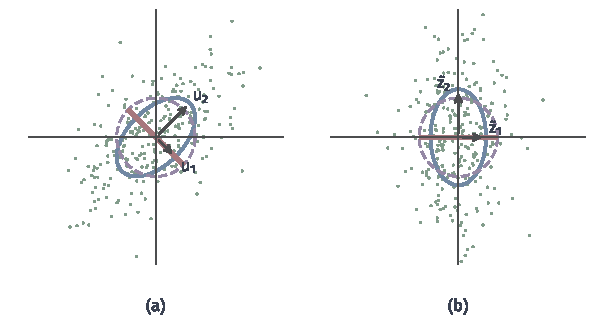
\includegraphics[width=104mm]{figures/07-probability/06-channel-coding/matplotlib/gcc-correlated-noise/figure.pdf}
 \caption{协方差为$\bm{\Sigma}=\bigl[\begin{smallmatrix}2&1\\1&2\end{smallmatrix}\bigr]$的噪声。绿点是$250$个噪声样本（种子$3$），蓝色椭圆是$\bm{z}^{\top}\bm{\Sigma}^{-1}\bm{z}=1$，黑色箭头是$\sqrt{\lambda_j}\bm{u}_j$，紫色虚线圆的半径是$\sqrt{P}=\sqrt2$，红色线段是最优输入沿$\bm{u}_1$方向的$\pm$一个标准差。(a)原坐标。(b)乘以$\bm{U}^{\top}$后的坐标，噪声分量独立，方差为$1$与$3$。}
 \label{fig:gcc-correlated-noise}
\end{BookInlineFigure}

\paragraph{白化}
另一种常见的处理是先把噪声变成单位协方差。接收端把输出乘以对称矩阵$\bm{\Sigma}^{-1/2}$，它与$\bm{\Sigma}$有相同的特征向量，特征值为$\lambda_j^{-1/2}$。这一操作称为白化：
\[
 \bar{\bm{Y}}=\bm{\Sigma}^{-1/2}\bm{Y}=\bm{\Sigma}^{-1/2}\bm{X}+\bm{N},\qquad \bm{N}=\bm{\Sigma}^{-1/2}\bm{Z}\sim\mathcal{N}(\bm{0},\bm{I}) .
\]
接收端的可逆变换可以随时撤销，不改变容量。但白化以后，信道的“输入”变成了$\bar{\bm{X}}=\bm{\Sigma}^{-1/2}\bm{X}$。若把$\bar{\bm{X}}$当作新的输入，信道是$\bar{\bm{Y}}=\bar{\bm{X}}+\bm{N}$，噪声是白的，预算却要跟着变：
\[
 \lVert\bm{X}\rVert_2^2=\lVert\bm{\Sigma}^{1/2}\bar{\bm{X}}\rVert_2^2=\bar{\bm{X}}^{\top}\bm{\Sigma}\bar{\bm{X}} .
\]
于是约束成为带权的预算
\begin{equation}
 \sum_{i=1}^{n}\bar{\bm{x}}_i^{\top}\bm{\Sigma}\bar{\bm{x}}_i\leq nP .
 \label{eq:gcc-weighted-budget}
\end{equation}
沿$\bm{u}_j$方向，$\bar{\bm{x}}$每单位平方长度要花$\lambda_j$单位的实际功率。

若忽略这一点，把白化后的问题当作单位噪声、欧氏预算的普通平行信道，注水会把功率平分，得到错误的答案。例中两个分量噪声都是$1$，平分预算$2$，得到
\[
 2\cdot\frac12\log_2(1+1)=1\ \text{比特},
\]
高于真正的容量$0.792$。多出来的部分来自一个不存在的便宜方向：沿$\bm{u}_2$放置的$\bar{\bm{x}}$实际要付三倍的功率。图~\ref{fig:gcc-whitening}画出白化后的坐标：噪声云变圆，真正的预算是紫色椭圆，错误的预算是黄色虚线圆。

\begin{BookInlineFigure}
 \centering
 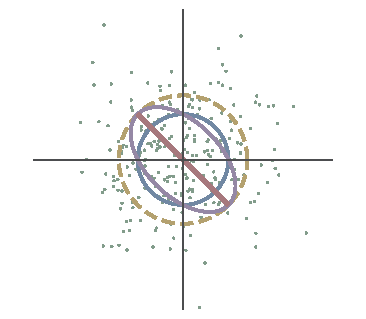
\includegraphics[width=62mm]{figures/07-probability/06-channel-coding/matplotlib/gcc-whitening/figure.pdf}
 \caption{白化后的坐标（与图~\ref{fig:gcc-correlated-noise}同一组噪声样本，绿点）。蓝圆是单位噪声的等高线；紫色椭圆是真正的预算$\bar{\bm{x}}^{\top}\bm{\Sigma}\bar{\bm{x}}\leq P$，沿$\bm{u}_1$的半轴为$\sqrt2$，沿$\bm{u}_2$的半轴为$\sqrt{2/3}$；黄色虚线圆是错误的预算$\lVert\bar{\bm{x}}\rVert_2^2\leq P$。红色线段是最优输入方向。}
 \label{fig:gcc-whitening}
\end{BookInlineFigure}

正确的做法有两种，结果相同。其一，保留原来的输入$\bm{X}$，把白化后的信道写成带增益的形式$\bar{\bm{Y}}=\bm{G}\bm{X}+\bm{N}$，$\bm{G}=\bm{\Sigma}^{-1/2}$。在特征向量坐标下，第$j$个分量是
\[
 \tilde{Y}_j=\lambda_j^{-1/2}\tilde{X}_j+N_j ,
\]
增益为$\lambda_j^{-1/2}$。两边乘以$\lambda_j^{1/2}$，得到$\tilde{X}_j$加上方差$\lambda_j$的噪声，回到对$\lambda_j$注水。其二，保留带权预算，把沿$\bm{u}_j$方向的白化输入功率记为$\bar{p}_j$，它的实际成本是$\lambda_j\bar{p}_j$，容量贡献是$\frac12\log_2(1+\bar{p}_j)$；令$P_j=\lambda_j\bar{p}_j$，问题又变成$\sum_j\frac12\log_2(1+P_j/\lambda_j)$在$\sum_jP_j\leq P$下的最大化。

\paragraph{一般的可逆变换}
上面的现象对任何可逆变换都成立。接收端的可逆变换不改变互信息，也不改变容量。发送端若用可逆矩阵$\bm{A}$换元，$\bm{X}=\bm{A}\bar{\bm{X}}$，预算中的$\lVert\bm{X}\rVert_2^2$就变成以$\bm{A}^{\top}\bm{A}$为矩阵的二次型；只有$\bm{A}$是正交矩阵时，$\bm{A}^{\top}\bm{A}=\bm{I}$，欧氏预算才保持原样。容量是“信道加约束”这一整体的性质，变换信道时必须同时变换约束。

同样的办法处理带增益矩阵的信道$\bm{Y}=\bm{H}\bm{X}+\bm{N}$，$\bm{H}$可逆，$\bm{N}\sim\mathcal{N}(\bm{0},\bm{I})$。由奇异值分解$\bm{H}=\bm{V}\bm{S}\bm{U}^{\top}$，发送端用$\bm{U}$、接收端用$\bm{V}^{\top}$，两者都是正交矩阵，信道化为增益为奇异值$s_j$的平行分量；每个分量除以增益后，等价于噪声方差为$1/s_j^2$的平行信道，再对$1/s_j^2$注水。

\paragraph{正定的作用}
定理要求$\bm{\Sigma}$正定。若$\bm{\Sigma}$有一个特征值为零，相应方向上没有噪声：沿这个方向发送任意实数，接收端在这个方向上的投影就是它本身，于是不同的实数都能被区分，容量为无穷。特征值很小但为正时，容量有限；这个方向的水底最低，注水时它最先分到功率。
